\documentclass[onecolumn, preprint]{sigplanconf}
\usepackage{multicol}
\usepackage{listings}
\usepackage{comment}
\usepackage{graphicx}
\usepackage{natbib}
\usepackage{amsmath}
%\usepackage[scaled=1.04]{couriers}

\newcommand{\select}[2]{\textsf{select } #1\ #2}
\newcommand{\store}[3]{\textsf{store } #1\ #2\ #3}
\newcommand{\loa}[2]{\textsf{list\_of\_array } #1\ #2}
\newcommand{\nth}[3]{\textsf{nth } #1\ #2\ #3}
\newcommand{\unth}[3]{\textsf{upd } #1\ #2\ #3}

\newcommand{\codeinl}[1]{\texttt{#1}}

\newcommand{\qfax}{\emph{QF\_AX}}
\newcommand\doubleplus{+\kern-1.3ex+\kern0.8ex}


\title{COS 597B: Final Report\\
\emph{Towards SMT in VST}}

\authorinfo{Santiago Cuellar \and Olivier Savary B\'{e}langer}
           {Princeton University}
           {scuellar/olivierb@princeton.edu}

\begin{document}
\maketitle


%start
\section{Introduction}
When formally proving the function correctness of programs, a portion of the proof or lemmas require a level of intuition or higher-order reasoning which goes beyond what is supported by automated theorem provers. However, between these crucial steps are many mechanical ones. Certain interactive theorem provers such as Coq provide scripting facilities to automate these steps, but this limited form of automation is ad hoc and brittle. It has been observed that many of these steps can be discharged by reasoning over SMT theories which can be performed by existing SMT solvers \citep{appelnote}. 

The \emph{Verified software Toolchain} is a powerful tool for verifying programs end-to-end. %More description 
The tool often produces subgoals over well studied theories with partial or full decision procedures, such as uninterpreted functions, theories of lists and theories of arrays.The goal of the project is to investigate using the power of modern SMT solvers to discharge obligations generated by VST. Our contributions are:
%After investigated the currently available tools to interface Coq and SMT solvers, we found out that SMTCoq \citep{keller13} already implements a pipeline from Coq goals to SMT-LIB \citep{smtlib}, a common format for SMT queries, and back into Coq after being solved by an SMT solver producing evidences. However, limitations in the current versions of SMTCoq, SMT-LIB and SMT solvers interfacing with SMT-LIB and SMTCoq prevent us from experimenting with this pipeline. Our contributions are:
\begin{itemize}
\item A short survey on the state of tools that can be used for connecting VST with an SMT solver (Sec.~\ref{sec:survey}). %wording
 \item Identifying goals in VST development which could be reduce to formulas in SMT theories (Sec.~\ref{sec:motiv})
 %\item Identifying the theories needed for such development to be useful %We only identify this for array, right?
 \item Sketching a completed pipeline assuming minimal updates to relevant tools (Sec.~\ref{sec:solution})
 \item Developping an encoding for list-reasoning to embed it in the theory of arrays with uninterpreted functions (\emph{QF\_AUFLIA}) (Sec.~\ref{sec:solution})
 \item Proving the soundness of the above encoding (Sec.~\ref{sec:proofs})
\end{itemize}

This report is organized as follow: Section 2 provide backgrounds about the tools and theories used in this project. Section 3 provides an overview of the solution, concentrating on the design of the encoding for supported list operations. Section 4 sketches proof of soundness of the encoding. Finally, section 5 explores future works for our project and discuss of the different assumption made of tools used.

\section{The Verified Software Toolchain}
\label{sec:VST}

The Verified Software Toolchain is a project developed at Princeton University\cite{VST}, which helps users verify, with machine-checked proofs, programs written in C with respect to their specifications written in Coq. The logic comes with an end-to-end proof assuring that the user verification proofs really hold in the machine-language program, running in the operating-system context. At the top level, \emph{VST} provides a separation logic to reason about pointer-manipulating programs and a \emph{Hoare logic} with full support for C control-flow and data-flow. 

Each of those components comes with partial automation, helping the user reason about her programs. In particular, VST provides tactics to reason about the control-flow of a program. The tactics produce subgoals in the form of consequence rules. VST provides automation to discharge spatial subgoals (that is dealing with pointers, in the separation logic), but when the subgoals are pure (i.e. not spatial), the user must prove them by hand. Such pure theorems are often about data-structure manipulation, functions or linear arithmetic and could greatly benefit from automation.


\section{Motivating Example: Swap}
\label{sec:motiv}

We will use the simple C program \texttt{swap} as a running example.

\begin{figure}
\begin{lstlisting}[language=C,basicstyle=\small,frame=none, tabsize=2, escapeinside={(*}{*)}]  % Start your code-block

void swap(int a[], int i, int j){
  int t1, t2;
  t1 = a[i];
  t2 = a[j];
  a[i] = t2;
  a[j] = t1;
}
\end{lstlisting}
   \label{fig:swap}
   \caption{The \texttt{swap}  C code}
\end{figure}

The function \texttt{swap} is a C function taking in an array \texttt{a} and two indices \texttt{i} and \texttt{j}. Assuming both index are in bounds, the function exchanges the contents of \texttt{a} at indices \texttt{i} and \texttt{j}, with the rest of \texttt{a} being left unchanged. We write the specification for this function as a Hoare triple in VST in figure \ref{fig:hoarswap} and we discuss the important parts.

\begin{figure}
\begin{lstlisting}[numbers=left, basicstyle=\small,frame=none, tabsize=2, escapeinside={(*}{*)}]  
Definition swap_spec :=
 DECLARE _swap
  WITH a: val, sh: share, contents: list int, i : Z, j : Z, size: Z
  PRE  [ _a OF (tptr tint), _i OF tint, _j OF tint  ]
  PROP(writable_share sh; 0 <= i < size;  0 <= j < size; 0 <= size <= Int.max_signed)
  LOCAL(temp _a a; temp _i (Vint (Int.repr i)); temp _j (Vint (Int.repr j)))
  SEP (data_at sh (tarray tint size) (map Vint contents) a)
  POST [ tvoid]
   EX contents': list int,
   PROP( \textbf{Znth i contents' Int.zero = Znth j contents Int.zero;
        Znth j contents' Int.zero = Znth i contents Int.zero;
        forall k, i<> k -> j<> k -> Znth k contents' Int.zero = Znth k contents Int.zero})
   LOCAL()
   SEP (data_at sh (tarray tint size) (map Vint contents') a).
\end{lstlisting}
\label{fig:hoarswap}
   \caption{The specification of \texttt{swap} in VST}
\end{figure}
Lines 4 through 7 represent the precondition starting with PRE. Line 5 requires the indices $i$ and $j$ to be in bound and the size of the array to be representable:
$$ 0 \leq i < size \wedge 0 \leq j < size  \wedge 0 \leq size \leq Int.max\_signed $$
Line 7 states the spatial constraints of the precondition. In this case, that there is an array of size $size$ at address $a$ and content $contents$. Lines 8 through 14, represent the postcondition, starting with POST. Line 14 ensures that, after execution, the the array at address $a$ has the same size, but new content $contents'$, quantified at line 9. Lines 10 through 12 are the most relevant for us: they specify the relationship between the initial and final contents of the array. Namely:
$$contents'[x] = \left\{\begin{array}{cc}contents[j] & x = i \\contents[i] & x = j \\contents[x] & otherwise\end{array}\right.$$

The automation of VST uses the sequence rule of Hoare logic
$$\{P\} c_1;c_2 \{S\}$$
and allows the user to step through the program, proving that every steps postcondition implies the next steps precondition. Finally, the user must prove that the resulting postcondition implies the postcondition of the specification. In the specific case of swap there are three final subgoals:


\begin{equation}
\label{sub1}
\begin{aligned}
&0 \leq i < size \rightarrow &\\
&0 \leq j < size \rightarrow &\\
&\textsf{length } contents' = size \rightarrow &\\
& \hspace{20pt} \nth i contents' \  0 = \nth j contents \ 0.
\end{aligned}
\end{equation}

\begin{equation}
\label{sub2}
\begin{aligned}
&0 \leq i < size \rightarrow &\\
&0 \leq j < size \rightarrow &\\
&\textsf{length } contents' = size \rightarrow &\\
& \hspace{20pt} \nth j contents' \  0 = \nth i contents \ 0.
\end{aligned}
\end{equation}

\begin{equation}
\label{sub3}
\begin{aligned}
&\forall k, k\not = i \rightarrow k\not =j & \\
&0 \leq i < size \rightarrow &\\
&0 \leq j < size \rightarrow &\\
&\textsf{length } contents' = size \rightarrow &\\
& \hspace{20pt} \nth k contents' \  0 = \nth k contents \ 0.
\end{aligned}
\end{equation}

Where $contents'$ is the content of the array $a$ after execution:
$$contents' = (\unth j (\unth i contents (\nth j contents \  0)) (\nth i contents \  0)).$$
The three subgoals require that $i$ and $j$ are within bounds, between 0 and the size of $contents'$. Subgoals \ref{sub1} and \ref{sub2} state that indices $i$ and $j$ are swaped.
Subgoal \ref{sub3} states that all other indices remain unchanged.

\

These kind of subgoals are not unique in any way. They are the kind of goals users see when verifying programs that read and write arrays, and these goals can be solved automatically by a modern SMT solver! Well, not immediately. As we will see, we need to properly encode the goals, to embed them into a know Modulo Theory. Also, we need to translate the the goal to an SMT friendly language, such as SMTlib. Then, we find a SMT solver that contains the desired theory. Finally, we must reflect back the resulting proof, by translating it into to coq. All of these steps must be proven sound, such that the produced proof is in fact a proof of the original goal. % include the number of sections or references 

In this project, we will explore all of this steps with a particular emphasis on the initial encoding and the soundness of it.





%While proving that the C code for swap respect this specification using VST, the following list-based side conditions are generated:

TODO


%All these conditions can be proven with simple but tedious proofs based solely on bounds reasoning and on the interaction between \texttt{Znth} and \texttt{upd_Znth}. In the remainder of this report, we will show how to automate these goals and more by using an automated theorem solver.



\section{Surveying the state of related tools}
\label{sec:survey}
% SMTCOQ
\subsection{SMT\_COQ}
\emph{SMT\_COQ} is a certified SMT interface for the Coq interactive theorem prover developed by Dr. Chantal Keller. It is built around a simple SMT solver proven-correct in Coq.
It works by encoding a Coq goal as an SMT formula, which may be proven valid by an external SMT solver. The SMT solver then generates a witness of the validity (for SAT, this witness would be the unsatisfiable core), which is validated by the simple SMT solver in Coq. Finally, the proof of correctness of this certified solver allows the reflection of the SMT decision in Coq, automatically solving the goal.

\emph{SMT\_COQ} currently only support the theory of uninterpreted functions \emph{QF\_UF} and the theory of linear arithmetic \emph{QF\_LIA}, and interfaces with the outmoded SMT solver VeriT, but it is planned to support the theory of arrays \emph{QF\_AX} and interface with \emph{CVC4} \citep{CVC4}, a state-of-the-art SMT solver.

\subsection{CVC4}
\emph{CVC4} is an efficient, open-source SMT solver which is in active development. It in relevant to us because of its planned support by \emph{SMT\_COQ}.

\emph{CVC4} already supports many theories including both the theory of arrays and the theory of datatypes. It however only generate proof witness for a limited subset of the theories, limited at the moment to simple, quantifier-free arithmetic theories. We are aware of work being done currenlt on  proof witness generation for \emph{QF\_AX}.


\section{Overview of our Solution}
\label{sec:solution}

In the remainder of this report, we present our solution which consist of encoding list operations as operation over arrays in various SMT theories. While simple operations such as \texttt{nth} and \texttt{upd\_nth} can be encoded in the quantifier-free fragment of the theory of array with uninterpreted functions and linear arithmetic \emph{QF\_AUFLIA}, other operations require stronger theories such as \emph{AUFLIA}. 

Targeting \emph{QF\_AUFLIA} is a pragmatic choice. While the theory of inductive datatypes would lead to a direct encoding of lists and list operations, its support is not planned for SMTCoq and would require significant extension to SMT-LIB and CVC4 (which supports the theory but does not generate proof witness for it). 

%dev
\subsection{A High-Level View of the Envisioned Machinery}
The following graphics describes the different components and the steps that goes into automatically proving an SMT goal using an SMT solver. Doted line represents works done by external tools, where full lines are specific to this project. 
\begin{center}
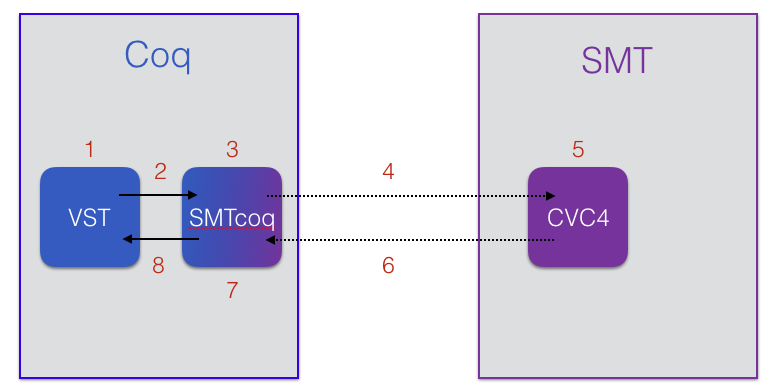
\includegraphics[scale=0.5]{pictures/arch.png}
\end{center}


\begin{enumerate}
\item %1
  A tactic provided by VST isolates the propositional portion of goals from separation-logic predicates.
\item %2
  The propositional goal is encoded into a Coq representation of a datatype which can be manipulated by SMT theories.
  
\item %3
 SMTCoq reifies the encoded goal as an OCaml datatype representing an SMT query equivalent to the encoded goal
  
\item %4
  SMTCoq generates an SMT-LIB from the OCaml reification of the goal, and send it to CVC4, an SMT solver
  
\item %5
  CVC4 either find a counter example to the query, in which case either the goal is false or it falls into the incomplete portion of the encoding, or it returns UNSAT together with a proof witness of the decision
  
\item %6
  Assuming an UNSAT decision (which asserts the validity of the initial goal), the proof witness is interpreted back in Coq 
  
  
\item %7
  The proof witness is verified by the certified SMT solver included in SMTCoq and the decision is reflected back in Coq as a proof of the encoded goal
  
\item %8
  By soundness of encoding, we use the validity of the encoded goal to prove the validity of the initial goal

  
\end{enumerate}

Due to current limitation of SMTCoq, in CVC4 and to time constraint, the work described in this report related to the following steps in the diagram:
\begin{itemize}
  \item $2$ to $4$ - encoding list goals as queries in the theory of arrays
  \item $8$ - proving the soundness of our encoding
\end{itemize}




% QF_AX, OF_AULIA and their support (and proof generation)
\subsection{The SMT Theory of Arrays}
The extensional theory of arrays is an SMT theory to reason about integer-indexed, infinite collection of elements. Arrays are accessed using function \texttt{select} of type \texttt{array $\rightarrow$ int $\rightarrow$ el} and modified with function \texttt{store} of type \texttt{array $\rightarrow$ int $\rightarrow$ el $\rightarrow$ array}. The simplest fragment of this theory is \emph{QF\_AX}. This quantifier-free theory is based on three axioms:
\begin{enumerate}
\item selecting from the last store:
  \begin{multicols}{2}
    
  $$ \forall a i, \textsf{select } (\textsf{store } a\ i\ e)\ i = e$$
which states that selecting returns what was last stored at that location
 
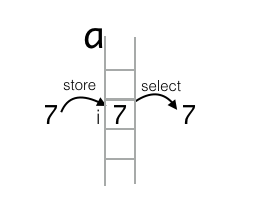
\includegraphics[scale=0.5]{pictures/axiom1.png}

  \end{multicols}
  
\item selecting from a previous store:
  \begin{multicols}{2}
  $$ \forall a i j, i \neq j \to \textsf{select } (\textsf{store } a\ j\ e)\ i = \textsf{select } a i$$
  which means that storing an element has not effect on what can be selected at other indices.

  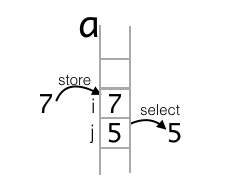
\includegraphics[scale=0.5]{pictures/axiom2.png}
  \end{multicols}
  
\item and extensionality:
  
  \begin{multicols}{2}
  $$ \forall a b, (\forall i, \textsf{select } a\ i = \textsf{select } b\ i) \to a = b$$
  which means that arrays which agrees on elements for every indices can be considered equal.

  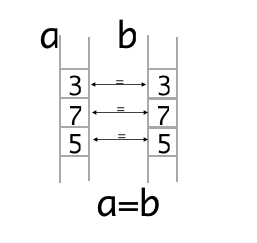
\includegraphics[scale=0.5]{pictures/axiom3.png}
  \end{multicols}
  \end{enumerate}
  

The theory of arrays can be augmented with uninterpreted functions and linear arithmetic (\emph{QF\_AUFLIA}) and to allow a limited form of quantification (\emph{AUFLIA})



\subsection{Encoding Lists as Arrays}

% difference between list and QF_AX
In Coq, lists are an inductive datatype representing an ordered collection of finitely many elements of a given type. 
\begin{lstlisting}
inductive list A : Set :=
 } nil : list A
 } cons : A -> list A -> list A.
\end{lstlisting}

In VST, C arrays are reasoned about propositionally as list, using total operation such as \texttt{upd\_Znth} and \texttt{nthZ}, using mathematical integers as index and a default value as argument to \texttt{nthZ} returned when accessing the array out of bound. 

As seen in the previous section, the arrays manipulated in \emph{QF\_AX} are associative arrays rather than programmatic ones. They represent an infinite collection of key-value pair where the keys are mathematical integers. 

The basis of our encoding is that the \emph{QF\_AX} array \texttt{a} representing Coq list \texttt{l} will be constrained to contain the same elements as \texttt{l} from indices $0$ to $\mathsf{length} l - 1$ and the default value $d$ otherwise.This means that it should always be the case that
$$ a_i = \textsf{nthZ}\ l\ i\ d$$

Given a goal about lists in VST, we first rewrite it in a three-address code fashion, binding the result of every list operation to a new variable. Then, each operation is encoded according a general, sound correspondence to operations in the theory of arrays:

% encoding of nth
For every goal of the form $s = \textsf{nthZ}\ i\ ls\ d$, we add the following in the conclusion on the formula sent to the SMT solver:

$$ (0 \leq j < \textsf{len}\ as) \to s = \textsf{select } as\ j\ \wedge$$
$$\neg (0 \leq j < \textsf{len}\ as) \to s = d $$

Where $as$ is an array corresponding to the list $ls$, and $len$ is an uninterpreted functions which will be constrained by hypothesis in the VST goal about $ls$'s boundaries.


% encoding of upd
$\textsf{upd\_Znth}$ is encoded almost directly by $AX$'s operation $\textsf{store}$. For every goal of the form $s = \textsf{upd\_Znth\ i\ e\ ls}$, we augment the formula with
$$ as' = \textsf{store}\ as\ i\ e \wedge 0 \leq i \leq \textsf{len}\ as \to \textsf{len}\ as' = \textsf{len}\ as$$
which encodes the update operation and the fact that updating within boundaries preserves the length of the list.


% encoding of append
just like $\textsf{nthZ}$, $\textsf{append}$ is encoded using $\textsf{select}$. For every goal of the form $ls = ls_1 ++ ls_2$, we add the following constraints:
$$(0 \leq j < \textsf{len}\ as1) \to \textsf{select}\ as1\ j = \textsf{select}\ as\ j \wedge $$
$$(\textsf{len}\ as1 \leq j < \textsf{len}\ as1 + \textsf{len}\ as2) \to \textsf{select}\ as2\ j = \textsf{select}\ as\ (\textsf{len}\ as1 + j)$$
Under this encoding, the result accessing the resulting array $as$ is equal to the first array $as1$ between $0$ and the length of the first list $ls_1$ and to the second array $as2$ between the length of the first list $ls_1$ and the length of the resulting list $ls$.




\section{Soundness of the Solution, or Reflecting Back on Lists}
\label{sec:proofs}
% explanation of proof needed for the big picture to work
While we strive for correctness of encoding, differences between lists
and the infinite arrays as manipulated by \emph{QF\_AX} makes such encoding difficult to achieve in general. 
Fortunately, we can instead use a simpler, sound but incomplete encoding, such that the validity 
of the encoding implies the validity of the original formula, but not the other way around.
In other word, some valid goals may result in invalid encodings, but valid encoding only arises from valid goals.

% say something about nat vs Z

% proof of soundness of encoding
%% QF_AX as Array GDT + Axioms
We encode the theory of arrays over an abstract datatype arrays. For simplicity, we use \texttt{nat} instead of \texttt{Z}.  
\begin{lstlisting}
  Variable array: forall {A:Type}, Type.
  Variable select: forall {A}, array A -> nat -> A.
  Variable store : forall {A}, array A -> nat -> A -> array A.
\end{lstlisting}
By representing arrays with \texttt{Variable array}, we ensure that the only way to observe or modify arrays is to use \texttt{select} or \texttt{store}.

We then assert the three axioms of \emph{QF\_AX} as assumption with the Coq keyword \texttt{Axiom}.

\begin{lstlisting}
Axiom QFAX1 : forall A a i (e:A),
   select (store a i e) i = e.  
Axiom QFAX2 : forall A a i j (e:A),
   i <> j -> select (store a i e) j = select a j.  
Axiom QFAX3 : forall A (a b: array A),
   (forall i, select a i = select b i) -> a = b.  
\end{lstlisting}

We then define a function which transport the arrays (on which something was proved using \emph{QF\_AX}) back to the lists manipulated by VST:

\begin{lstlisting}
  Fixpoint list_of_array'' {A} L (ar:array A) :=
  match L with
    }  0 => nil
    } S n => (select ar (L))::(list_of_array'' n ar)
  end.


Definition list_of_array {A} i (ar:array A) :=
   List.rev (list_of_array'' i ar).
\end{lstlisting}




%% nth as select

\subsection{\texttt{nth}}
We prove our encoding of \texttt{nth} sound in theorem \texttt{enc\_nth}, which is stated as follow:
\begin{align*}
 & (\forall j, (0 \leq j < L) \to s = \select{ar}{j}) \to \\
 & (\forall j, (j \leq 0 \vee L \leq j) \to s = d) \to \\
 & s = \nth{i}{\loa{L}{ar}}{d} 
\end{align*}

The proof goes by induction on \codeinl{L}, with simple reasoning about the length of $\textsf{list\_of\_array}$ and on the behavior of function \textsf{nth} on overflow.

\begin{comment}
\begin{lstlisting}
Theorem enc_nth: forall A  L j (ar:array A) (ls:list A) (s:A)  (d:A),
  ((0 <= j < L) -> s = select ar j) /\
  (( j < 0 \/ L <= j) -> s = d) ->
  (s = nth j (list_of_array L ar) d).
\end{lstlisting}
\end{comment}





%% upd_nth as store
\subsection{\texttt{upd\_nth}}
We then prove that in-bound \texttt{store} encodes \texttt{upd\_nth} in theorem \texttt{enc\_upd}, stated as follow:

\begin{align*}
  (\forall i, (0 \leq i < L) \to ss = \store{ss}{i}{a}) \to 
     \loa{L}{ss'} &= \unth{i}{\loa{L}{ss}}{a}
\end{align*}

The proof is based on two lemmas, \texttt{enc\_upd\_ge} and \texttt{enc\_upd\_le} depending on if the update is done within the list's bound or not. Each lemmas are proven by induction on L.


\begin{comment}
\begin{lstlisting}
Theorem enc_upd: forall A i ss (a: array A) L ss',
   0 <= i < L
   ss' = store ss i a ->
   list_of_array L ss' = upd_nth i (list_of_array L ss) a.
\end{lstlisting}
\end{comment}


%% ++ as branch-and-select
\subsection{$\doubleplus$}
Finally, we prove that branching \codeinl{select} produces a sound encoding for list-append in theorem \texttt{enc\_app}, stated as follow:

\begin{align*}
(\forall i, (0 \leq i < L_1) \to \select{ss_1}{i} = \select{ss_3}{i}) &\to \\
  (\forall i, (0 \leq i < L_2) \to \select{ss_2}{i} = \select{ss_3}{i + L_1}) &\to  \\
  (\loa{L_1}{ss_1} \doubleplus \loa{L_2}{ss_2} &= \loa{L_1 + L_2}{ss_3}
\end{align*}

\begin{comment}
\begin{lstlisting}
Theorem enc_app: forall  A L1 L2 (ss1 ss2 ss3: array A),
                   (forall i, (0 <= i < L1)%nat -> select  ss1 i = select  ss3 i) ->
                   (forall i, (0 <= i < L2)%nat -> select ss2 i = select ss3 (i + L1)) ->
                   (list_of_array L1 ss1) ++ (list_of_array L2 ss2)  = list_of_array (L1+L2) ss3.
\end{lstlisting}
\end{comment}

The proof follows by induction on $L_2$ and reasoning about $\doubleplus$ and \texttt{rev}.


%end
\section{Future Work}
\label{sec:future}
% 4 pages just there
In the near future, we expect most of the current limitations to our work due to external tools to be lifted.

In order for the pipeline described in the previous sections to be completed, we need CVC4 to generate witnesses for the theory of arrays and SMTcoq to support the theory of arrays and to interface with CVC4. We have the confirmation from the developer of CVC4 and SMTcoq that these are being worked on. In the future, supports for more theories, especially quantified arrays and inductive datatypes, would permit for more direct encodings and, in the case of the latter, automatic generation of encoding together with correctness proof for the datatype and simple functions.


% supporting more list operations and potentially other datatypes
In the meantime, we can extend our encodings with more lists operations, potentially using \emph{AUFLIA} rather than its quantifier-free fragment \emph{QF\_AUFLIA}.

\section{Conclusion}
\label{sec:conclusion}
Our project is meant to be taken as an investigation of the realizability of harnessing an SMT solver to provide automate software verification goals in an interactive theorem prover such as Coq. We conclude that while architecturally we know how to assemble an interface such as this one, the tools which are currently available are too limited for realistic usage.




Even assuming \emph{SMT\_COQ}'s support for CVC4, and CVC4 proof generation for \emph{AUFLIA}, we doubt that our encoding of list goals as array will scale well to more list operations and goals about other inductive datatypes, and that it would be more practical than using the automation facilities already present in Coq. In a more distant future, we envision the support for the theory of inductive datatypes to be of high importance, as it would permit (and potentially generate automatically)  direct encoding of simple Coq datatypes, towards a seamless integration of SMT for VST.

\bibliography{bibi}
\bibliographystyle{abbrvnat}
\end{document}
